\documentclass[margin=2mm]{standalone}
\usepackage{tikz}
\usepackage{amsmath,amssymb,mathtools}
\begin{document}
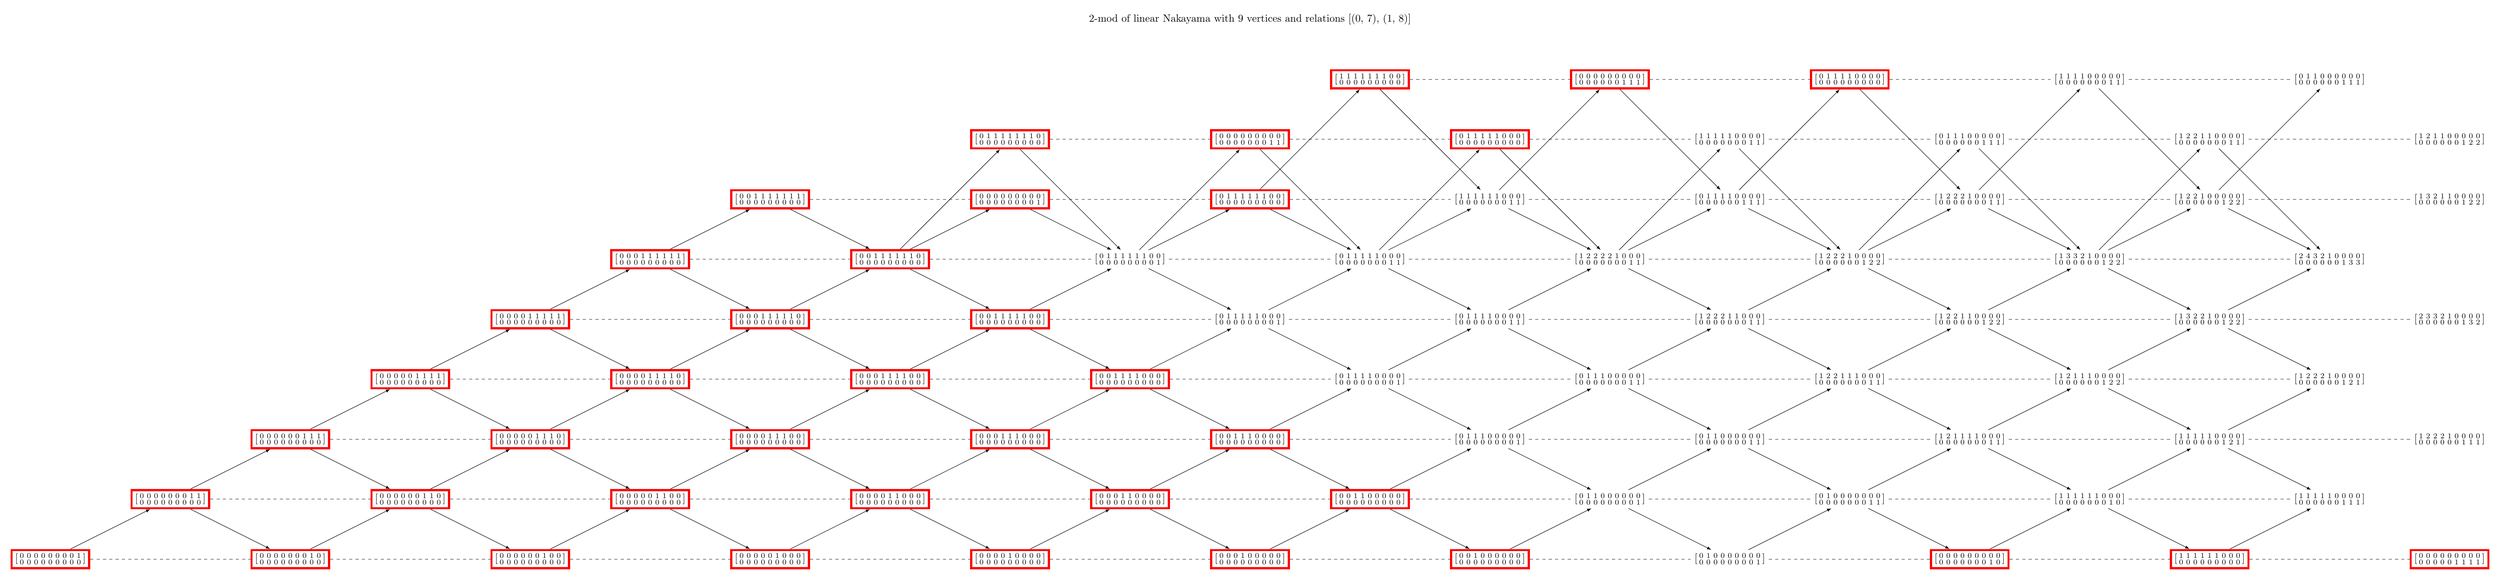
\begin{tikzpicture}[xscale=4,yscale=2]
\node at (10.0,9) [] {$2$-mod of linear Nakayama with 9 vertices and relations [(0, 7), (1, 8)]};
\node (t-0P0) at (11,8) [scale=1,rectangle,draw=red,line width=2pt] {$\begin{bsmallmatrix}
 1 & 1 & 1 & 1 & 1 & 1 & 1 & 0 & 0\\
 0 & 0 & 0 & 0 & 0 & 0 & 0 & 0 & 0\\
\end{bsmallmatrix}$};
\node (t-1P0) at (13,8) [scale=1,rectangle,draw=red,line width=2pt] {$\begin{bsmallmatrix}
 0 & 0 & 0 & 0 & 0 & 0 & 0 & 0 & 0\\
 0 & 0 & 0 & 0 & 0 & 0 & 1 & 1 & 1\\
\end{bsmallmatrix}$};
\node (t-2P0) at (15,8) [scale=1,rectangle,draw=red,line width=2pt] {$\begin{bsmallmatrix}
 0 & 1 & 1 & 1 & 1 & 0 & 0 & 0 & 0\\
 0 & 0 & 0 & 0 & 0 & 0 & 0 & 0 & 0\\
\end{bsmallmatrix}$};
\node (t-3P0) at (17,8) [scale=1] {$\begin{bsmallmatrix}
 1 & 1 & 1 & 1 & 0 & 0 & 0 & 0 & 0\\
 0 & 0 & 0 & 0 & 0 & 0 & 0 & 1 & 1\\
\end{bsmallmatrix}$};
\node (t-4P0) at (19,8) [scale=1] {$\begin{bsmallmatrix}
 0 & 1 & 1 & 0 & 0 & 0 & 0 & 0 & 0\\
 0 & 0 & 0 & 0 & 0 & 0 & 1 & 1 & 1\\
\end{bsmallmatrix}$};
\node (t-0P1) at (8,7) [scale=1,rectangle,draw=red,line width=2pt] {$\begin{bsmallmatrix}
 0 & 1 & 1 & 1 & 1 & 1 & 1 & 1 & 0\\
 0 & 0 & 0 & 0 & 0 & 0 & 0 & 0 & 0\\
\end{bsmallmatrix}$};
\node (t-1P1) at (10,7) [scale=1,rectangle,draw=red,line width=2pt] {$\begin{bsmallmatrix}
 0 & 0 & 0 & 0 & 0 & 0 & 0 & 0 & 0\\
 0 & 0 & 0 & 0 & 0 & 0 & 0 & 1 & 1\\
\end{bsmallmatrix}$};
\node (t-2P1) at (12,7) [scale=1,rectangle,draw=red,line width=2pt] {$\begin{bsmallmatrix}
 0 & 1 & 1 & 1 & 1 & 1 & 0 & 0 & 0\\
 0 & 0 & 0 & 0 & 0 & 0 & 0 & 0 & 0\\
\end{bsmallmatrix}$};
\node (t-3P1) at (14,7) [scale=1] {$\begin{bsmallmatrix}
 1 & 1 & 1 & 1 & 1 & 0 & 0 & 0 & 0\\
 0 & 0 & 0 & 0 & 0 & 0 & 0 & 1 & 1\\
\end{bsmallmatrix}$};
\node (t-4P1) at (16,7) [scale=1] {$\begin{bsmallmatrix}
 0 & 1 & 1 & 1 & 0 & 0 & 0 & 0 & 0\\
 0 & 0 & 0 & 0 & 0 & 0 & 1 & 1 & 1\\
\end{bsmallmatrix}$};
\node (t-5P1) at (18,7) [scale=1] {$\begin{bsmallmatrix}
 1 & 2 & 2 & 1 & 1 & 0 & 0 & 0 & 0\\
 0 & 0 & 0 & 0 & 0 & 0 & 0 & 1 & 1\\
\end{bsmallmatrix}$};
\node (t-6P1) at (20,7) [scale=1] {$\begin{bsmallmatrix}
 1 & 2 & 1 & 1 & 0 & 0 & 0 & 0 & 0\\
 0 & 0 & 0 & 0 & 0 & 0 & 1 & 2 & 2\\
\end{bsmallmatrix}$};
\node (t-0P2) at (6,6) [scale=1,rectangle,draw=red,line width=2pt] {$\begin{bsmallmatrix}
 0 & 0 & 1 & 1 & 1 & 1 & 1 & 1 & 1\\
 0 & 0 & 0 & 0 & 0 & 0 & 0 & 0 & 0\\
\end{bsmallmatrix}$};
\node (t-1P2) at (8,6) [scale=1,rectangle,draw=red,line width=2pt] {$\begin{bsmallmatrix}
 0 & 0 & 0 & 0 & 0 & 0 & 0 & 0 & 0\\
 0 & 0 & 0 & 0 & 0 & 0 & 0 & 0 & 1\\
\end{bsmallmatrix}$};
\node (t-2P2) at (10,6) [scale=1,rectangle,draw=red,line width=2pt] {$\begin{bsmallmatrix}
 0 & 1 & 1 & 1 & 1 & 1 & 1 & 0 & 0\\
 0 & 0 & 0 & 0 & 0 & 0 & 0 & 0 & 0\\
\end{bsmallmatrix}$};
\node (t-3P2) at (12,6) [scale=1] {$\begin{bsmallmatrix}
 1 & 1 & 1 & 1 & 1 & 1 & 0 & 0 & 0\\
 0 & 0 & 0 & 0 & 0 & 0 & 0 & 1 & 1\\
\end{bsmallmatrix}$};
\node (t-4P2) at (14,6) [scale=1] {$\begin{bsmallmatrix}
 0 & 1 & 1 & 1 & 1 & 0 & 0 & 0 & 0\\
 0 & 0 & 0 & 0 & 0 & 0 & 1 & 1 & 1\\
\end{bsmallmatrix}$};
\node (t-5P2) at (16,6) [scale=1] {$\begin{bsmallmatrix}
 1 & 2 & 2 & 2 & 1 & 0 & 0 & 0 & 0\\
 0 & 0 & 0 & 0 & 0 & 0 & 0 & 1 & 1\\
\end{bsmallmatrix}$};
\node (t-6P2) at (18,6) [scale=1] {$\begin{bsmallmatrix}
 1 & 2 & 2 & 1 & 0 & 0 & 0 & 0 & 0\\
 0 & 0 & 0 & 0 & 0 & 0 & 1 & 2 & 2\\
\end{bsmallmatrix}$};
\node (t-7P2) at (20,6) [scale=1] {$\begin{bsmallmatrix}
 1 & 3 & 2 & 1 & 1 & 0 & 0 & 0 & 0\\
 0 & 0 & 0 & 0 & 0 & 0 & 1 & 2 & 2\\
\end{bsmallmatrix}$};
\node (t-0P3) at (5,5) [scale=1,rectangle,draw=red,line width=2pt] {$\begin{bsmallmatrix}
 0 & 0 & 0 & 1 & 1 & 1 & 1 & 1 & 1\\
 0 & 0 & 0 & 0 & 0 & 0 & 0 & 0 & 0\\
\end{bsmallmatrix}$};
\node (t-1P3) at (7,5) [scale=1,rectangle,draw=red,line width=2pt] {$\begin{bsmallmatrix}
 0 & 0 & 1 & 1 & 1 & 1 & 1 & 1 & 0\\
 0 & 0 & 0 & 0 & 0 & 0 & 0 & 0 & 0\\
\end{bsmallmatrix}$};
\node (t-2P3) at (9,5) [scale=1] {$\begin{bsmallmatrix}
 0 & 1 & 1 & 1 & 1 & 1 & 1 & 0 & 0\\
 0 & 0 & 0 & 0 & 0 & 0 & 0 & 0 & 1\\
\end{bsmallmatrix}$};
\node (t-3P3) at (11,5) [scale=1] {$\begin{bsmallmatrix}
 0 & 1 & 1 & 1 & 1 & 1 & 0 & 0 & 0\\
 0 & 0 & 0 & 0 & 0 & 0 & 0 & 1 & 1\\
\end{bsmallmatrix}$};
\node (t-4P3) at (13,5) [scale=1] {$\begin{bsmallmatrix}
 1 & 2 & 2 & 2 & 2 & 1 & 0 & 0 & 0\\
 0 & 0 & 0 & 0 & 0 & 0 & 0 & 1 & 1\\
\end{bsmallmatrix}$};
\node (t-5P3) at (15,5) [scale=1] {$\begin{bsmallmatrix}
 1 & 2 & 2 & 2 & 1 & 0 & 0 & 0 & 0\\
 0 & 0 & 0 & 0 & 0 & 0 & 1 & 2 & 2\\
\end{bsmallmatrix}$};
\node (t-6P3) at (17,5) [scale=1] {$\begin{bsmallmatrix}
 1 & 3 & 3 & 2 & 1 & 0 & 0 & 0 & 0\\
 0 & 0 & 0 & 0 & 0 & 0 & 1 & 2 & 2\\
\end{bsmallmatrix}$};
\node (t-7P3) at (19,5) [scale=1] {$\begin{bsmallmatrix}
 2 & 4 & 3 & 2 & 1 & 0 & 0 & 0 & 0\\
 0 & 0 & 0 & 0 & 0 & 0 & 1 & 3 & 3\\
\end{bsmallmatrix}$};
\node (t-0P4) at (4,4) [scale=1,rectangle,draw=red,line width=2pt] {$\begin{bsmallmatrix}
 0 & 0 & 0 & 0 & 1 & 1 & 1 & 1 & 1\\
 0 & 0 & 0 & 0 & 0 & 0 & 0 & 0 & 0\\
\end{bsmallmatrix}$};
\node (t-1P4) at (6,4) [scale=1,rectangle,draw=red,line width=2pt] {$\begin{bsmallmatrix}
 0 & 0 & 0 & 1 & 1 & 1 & 1 & 1 & 0\\
 0 & 0 & 0 & 0 & 0 & 0 & 0 & 0 & 0\\
\end{bsmallmatrix}$};
\node (t-2P4) at (8,4) [scale=1,rectangle,draw=red,line width=2pt] {$\begin{bsmallmatrix}
 0 & 0 & 1 & 1 & 1 & 1 & 1 & 0 & 0\\
 0 & 0 & 0 & 0 & 0 & 0 & 0 & 0 & 0\\
\end{bsmallmatrix}$};
\node (t-3P4) at (10,4) [scale=1] {$\begin{bsmallmatrix}
 0 & 1 & 1 & 1 & 1 & 1 & 0 & 0 & 0\\
 0 & 0 & 0 & 0 & 0 & 0 & 0 & 0 & 1\\
\end{bsmallmatrix}$};
\node (t-4P4) at (12,4) [scale=1] {$\begin{bsmallmatrix}
 0 & 1 & 1 & 1 & 1 & 0 & 0 & 0 & 0\\
 0 & 0 & 0 & 0 & 0 & 0 & 0 & 1 & 1\\
\end{bsmallmatrix}$};
\node (t-5P4) at (14,4) [scale=1] {$\begin{bsmallmatrix}
 1 & 2 & 2 & 2 & 1 & 1 & 0 & 0 & 0\\
 0 & 0 & 0 & 0 & 0 & 0 & 0 & 1 & 1\\
\end{bsmallmatrix}$};
\node (t-6P4) at (16,4) [scale=1] {$\begin{bsmallmatrix}
 1 & 2 & 2 & 1 & 1 & 0 & 0 & 0 & 0\\
 0 & 0 & 0 & 0 & 0 & 0 & 1 & 2 & 2\\
\end{bsmallmatrix}$};
\node (t-7P4) at (18,4) [scale=1] {$\begin{bsmallmatrix}
 1 & 3 & 2 & 2 & 1 & 0 & 0 & 0 & 0\\
 0 & 0 & 0 & 0 & 0 & 0 & 1 & 2 & 2\\
\end{bsmallmatrix}$};
\node (t-8P4) at (20,4) [scale=1] {$\begin{bsmallmatrix}
 2 & 3 & 3 & 2 & 1 & 0 & 0 & 0 & 0\\
 0 & 0 & 0 & 0 & 0 & 0 & 1 & 3 & 2\\
\end{bsmallmatrix}$};
\node (t-0P5) at (3,3) [scale=1,rectangle,draw=red,line width=2pt] {$\begin{bsmallmatrix}
 0 & 0 & 0 & 0 & 0 & 1 & 1 & 1 & 1\\
 0 & 0 & 0 & 0 & 0 & 0 & 0 & 0 & 0\\
\end{bsmallmatrix}$};
\node (t-1P5) at (5,3) [scale=1,rectangle,draw=red,line width=2pt] {$\begin{bsmallmatrix}
 0 & 0 & 0 & 0 & 1 & 1 & 1 & 1 & 0\\
 0 & 0 & 0 & 0 & 0 & 0 & 0 & 0 & 0\\
\end{bsmallmatrix}$};
\node (t-2P5) at (7,3) [scale=1,rectangle,draw=red,line width=2pt] {$\begin{bsmallmatrix}
 0 & 0 & 0 & 1 & 1 & 1 & 1 & 0 & 0\\
 0 & 0 & 0 & 0 & 0 & 0 & 0 & 0 & 0\\
\end{bsmallmatrix}$};
\node (t-3P5) at (9,3) [scale=1,rectangle,draw=red,line width=2pt] {$\begin{bsmallmatrix}
 0 & 0 & 1 & 1 & 1 & 1 & 0 & 0 & 0\\
 0 & 0 & 0 & 0 & 0 & 0 & 0 & 0 & 0\\
\end{bsmallmatrix}$};
\node (t-4P5) at (11,3) [scale=1] {$\begin{bsmallmatrix}
 0 & 1 & 1 & 1 & 1 & 0 & 0 & 0 & 0\\
 0 & 0 & 0 & 0 & 0 & 0 & 0 & 0 & 1\\
\end{bsmallmatrix}$};
\node (t-5P5) at (13,3) [scale=1] {$\begin{bsmallmatrix}
 0 & 1 & 1 & 1 & 0 & 0 & 0 & 0 & 0\\
 0 & 0 & 0 & 0 & 0 & 0 & 0 & 1 & 1\\
\end{bsmallmatrix}$};
\node (t-6P5) at (15,3) [scale=1] {$\begin{bsmallmatrix}
 1 & 2 & 2 & 1 & 1 & 1 & 0 & 0 & 0\\
 0 & 0 & 0 & 0 & 0 & 0 & 0 & 1 & 1\\
\end{bsmallmatrix}$};
\node (t-7P5) at (17,3) [scale=1] {$\begin{bsmallmatrix}
 1 & 2 & 1 & 1 & 1 & 0 & 0 & 0 & 0\\
 0 & 0 & 0 & 0 & 0 & 0 & 1 & 2 & 2\\
\end{bsmallmatrix}$};
\node (t-8P5) at (19,3) [scale=1] {$\begin{bsmallmatrix}
 1 & 2 & 2 & 2 & 1 & 0 & 0 & 0 & 0\\
 0 & 0 & 0 & 0 & 0 & 0 & 1 & 2 & 1\\
\end{bsmallmatrix}$};
\node (t-0P6) at (2,2) [scale=1,rectangle,draw=red,line width=2pt] {$\begin{bsmallmatrix}
 0 & 0 & 0 & 0 & 0 & 0 & 1 & 1 & 1\\
 0 & 0 & 0 & 0 & 0 & 0 & 0 & 0 & 0\\
\end{bsmallmatrix}$};
\node (t-1P6) at (4,2) [scale=1,rectangle,draw=red,line width=2pt] {$\begin{bsmallmatrix}
 0 & 0 & 0 & 0 & 0 & 1 & 1 & 1 & 0\\
 0 & 0 & 0 & 0 & 0 & 0 & 0 & 0 & 0\\
\end{bsmallmatrix}$};
\node (t-2P6) at (6,2) [scale=1,rectangle,draw=red,line width=2pt] {$\begin{bsmallmatrix}
 0 & 0 & 0 & 0 & 1 & 1 & 1 & 0 & 0\\
 0 & 0 & 0 & 0 & 0 & 0 & 0 & 0 & 0\\
\end{bsmallmatrix}$};
\node (t-3P6) at (8,2) [scale=1,rectangle,draw=red,line width=2pt] {$\begin{bsmallmatrix}
 0 & 0 & 0 & 1 & 1 & 1 & 0 & 0 & 0\\
 0 & 0 & 0 & 0 & 0 & 0 & 0 & 0 & 0\\
\end{bsmallmatrix}$};
\node (t-4P6) at (10,2) [scale=1,rectangle,draw=red,line width=2pt] {$\begin{bsmallmatrix}
 0 & 0 & 1 & 1 & 1 & 0 & 0 & 0 & 0\\
 0 & 0 & 0 & 0 & 0 & 0 & 0 & 0 & 0\\
\end{bsmallmatrix}$};
\node (t-5P6) at (12,2) [scale=1] {$\begin{bsmallmatrix}
 0 & 1 & 1 & 1 & 0 & 0 & 0 & 0 & 0\\
 0 & 0 & 0 & 0 & 0 & 0 & 0 & 0 & 1\\
\end{bsmallmatrix}$};
\node (t-6P6) at (14,2) [scale=1] {$\begin{bsmallmatrix}
 0 & 1 & 1 & 0 & 0 & 0 & 0 & 0 & 0\\
 0 & 0 & 0 & 0 & 0 & 0 & 0 & 1 & 1\\
\end{bsmallmatrix}$};
\node (t-7P6) at (16,2) [scale=1] {$\begin{bsmallmatrix}
 1 & 2 & 1 & 1 & 1 & 1 & 0 & 0 & 0\\
 0 & 0 & 0 & 0 & 0 & 0 & 0 & 1 & 1\\
\end{bsmallmatrix}$};
\node (t-8P6) at (18,2) [scale=1] {$\begin{bsmallmatrix}
 1 & 1 & 1 & 1 & 1 & 0 & 0 & 0 & 0\\
 0 & 0 & 0 & 0 & 0 & 0 & 1 & 2 & 1\\
\end{bsmallmatrix}$};
\node (t-9P6) at (20,2) [scale=1] {$\begin{bsmallmatrix}
 1 & 2 & 2 & 2 & 1 & 0 & 0 & 0 & 0\\
 0 & 0 & 0 & 0 & 0 & 0 & 1 & 1 & 1\\
\end{bsmallmatrix}$};
\node (t-0P7) at (1,1) [scale=1,rectangle,draw=red,line width=2pt] {$\begin{bsmallmatrix}
 0 & 0 & 0 & 0 & 0 & 0 & 0 & 1 & 1\\
 0 & 0 & 0 & 0 & 0 & 0 & 0 & 0 & 0\\
\end{bsmallmatrix}$};
\node (t-1P7) at (3,1) [scale=1,rectangle,draw=red,line width=2pt] {$\begin{bsmallmatrix}
 0 & 0 & 0 & 0 & 0 & 0 & 1 & 1 & 0\\
 0 & 0 & 0 & 0 & 0 & 0 & 0 & 0 & 0\\
\end{bsmallmatrix}$};
\node (t-2P7) at (5,1) [scale=1,rectangle,draw=red,line width=2pt] {$\begin{bsmallmatrix}
 0 & 0 & 0 & 0 & 0 & 1 & 1 & 0 & 0\\
 0 & 0 & 0 & 0 & 0 & 0 & 0 & 0 & 0\\
\end{bsmallmatrix}$};
\node (t-3P7) at (7,1) [scale=1,rectangle,draw=red,line width=2pt] {$\begin{bsmallmatrix}
 0 & 0 & 0 & 0 & 1 & 1 & 0 & 0 & 0\\
 0 & 0 & 0 & 0 & 0 & 0 & 0 & 0 & 0\\
\end{bsmallmatrix}$};
\node (t-4P7) at (9,1) [scale=1,rectangle,draw=red,line width=2pt] {$\begin{bsmallmatrix}
 0 & 0 & 0 & 1 & 1 & 0 & 0 & 0 & 0\\
 0 & 0 & 0 & 0 & 0 & 0 & 0 & 0 & 0\\
\end{bsmallmatrix}$};
\node (t-5P7) at (11,1) [scale=1,rectangle,draw=red,line width=2pt] {$\begin{bsmallmatrix}
 0 & 0 & 1 & 1 & 0 & 0 & 0 & 0 & 0\\
 0 & 0 & 0 & 0 & 0 & 0 & 0 & 0 & 0\\
\end{bsmallmatrix}$};
\node (t-6P7) at (13,1) [scale=1] {$\begin{bsmallmatrix}
 0 & 1 & 1 & 0 & 0 & 0 & 0 & 0 & 0\\
 0 & 0 & 0 & 0 & 0 & 0 & 0 & 0 & 1\\
\end{bsmallmatrix}$};
\node (t-7P7) at (15,1) [scale=1] {$\begin{bsmallmatrix}
 0 & 1 & 0 & 0 & 0 & 0 & 0 & 0 & 0\\
 0 & 0 & 0 & 0 & 0 & 0 & 0 & 1 & 1\\
\end{bsmallmatrix}$};
\node (t-8P7) at (17,1) [scale=1] {$\begin{bsmallmatrix}
 1 & 1 & 1 & 1 & 1 & 1 & 0 & 0 & 0\\
 0 & 0 & 0 & 0 & 0 & 0 & 0 & 1 & 0\\
\end{bsmallmatrix}$};
\node (t-9P7) at (19,1) [scale=1] {$\begin{bsmallmatrix}
 1 & 1 & 1 & 1 & 1 & 0 & 0 & 0 & 0\\
 0 & 0 & 0 & 0 & 0 & 0 & 1 & 1 & 1\\
\end{bsmallmatrix}$};
\node (t-0P8) at (0,0) [scale=1,rectangle,draw=red,line width=2pt] {$\begin{bsmallmatrix}
 0 & 0 & 0 & 0 & 0 & 0 & 0 & 0 & 1\\
 0 & 0 & 0 & 0 & 0 & 0 & 0 & 0 & 0\\
\end{bsmallmatrix}$};
\node (t-1P8) at (2,0) [scale=1,rectangle,draw=red,line width=2pt] {$\begin{bsmallmatrix}
 0 & 0 & 0 & 0 & 0 & 0 & 0 & 1 & 0\\
 0 & 0 & 0 & 0 & 0 & 0 & 0 & 0 & 0\\
\end{bsmallmatrix}$};
\node (t-2P8) at (4,0) [scale=1,rectangle,draw=red,line width=2pt] {$\begin{bsmallmatrix}
 0 & 0 & 0 & 0 & 0 & 0 & 1 & 0 & 0\\
 0 & 0 & 0 & 0 & 0 & 0 & 0 & 0 & 0\\
\end{bsmallmatrix}$};
\node (t-3P8) at (6,0) [scale=1,rectangle,draw=red,line width=2pt] {$\begin{bsmallmatrix}
 0 & 0 & 0 & 0 & 0 & 1 & 0 & 0 & 0\\
 0 & 0 & 0 & 0 & 0 & 0 & 0 & 0 & 0\\
\end{bsmallmatrix}$};
\node (t-4P8) at (8,0) [scale=1,rectangle,draw=red,line width=2pt] {$\begin{bsmallmatrix}
 0 & 0 & 0 & 0 & 1 & 0 & 0 & 0 & 0\\
 0 & 0 & 0 & 0 & 0 & 0 & 0 & 0 & 0\\
\end{bsmallmatrix}$};
\node (t-5P8) at (10,0) [scale=1,rectangle,draw=red,line width=2pt] {$\begin{bsmallmatrix}
 0 & 0 & 0 & 1 & 0 & 0 & 0 & 0 & 0\\
 0 & 0 & 0 & 0 & 0 & 0 & 0 & 0 & 0\\
\end{bsmallmatrix}$};
\node (t-6P8) at (12,0) [scale=1,rectangle,draw=red,line width=2pt] {$\begin{bsmallmatrix}
 0 & 0 & 1 & 0 & 0 & 0 & 0 & 0 & 0\\
 0 & 0 & 0 & 0 & 0 & 0 & 0 & 0 & 0\\
\end{bsmallmatrix}$};
\node (t-7P8) at (14,0) [scale=1] {$\begin{bsmallmatrix}
 0 & 1 & 0 & 0 & 0 & 0 & 0 & 0 & 0\\
 0 & 0 & 0 & 0 & 0 & 0 & 0 & 0 & 1\\
\end{bsmallmatrix}$};
\node (t-8P8) at (16,0) [scale=1,rectangle,draw=red,line width=2pt] {$\begin{bsmallmatrix}
 0 & 0 & 0 & 0 & 0 & 0 & 0 & 0 & 0\\
 0 & 0 & 0 & 0 & 0 & 0 & 0 & 1 & 0\\
\end{bsmallmatrix}$};
\node (t-9P8) at (18,0) [scale=1,rectangle,draw=red,line width=2pt] {$\begin{bsmallmatrix}
 1 & 1 & 1 & 1 & 1 & 1 & 0 & 0 & 0\\
 0 & 0 & 0 & 0 & 0 & 0 & 0 & 0 & 0\\
\end{bsmallmatrix}$};
\node (t-10P8) at (20,0) [scale=1,rectangle,draw=red,line width=2pt] {$\begin{bsmallmatrix}
 0 & 0 & 0 & 0 & 0 & 0 & 0 & 0 & 0\\
 0 & 0 & 0 & 0 & 0 & 1 & 1 & 1 & 1\\
\end{bsmallmatrix}$};
\draw[-latex] (t-0P0) -- (t-3P2);
\draw[-latex] (t-1P0) -- (t-4P2);
\draw[-latex] (t-2P0) -- (t-5P2);
\draw[-latex] (t-3P0) -- (t-6P2);
\draw[-latex] (t-0P1) -- (t-2P3);
\draw[-latex] (t-1P1) -- (t-3P3);
\draw[-latex] (t-2P1) -- (t-4P3);
\draw[-latex] (t-3P1) -- (t-5P3);
\draw[-latex] (t-4P1) -- (t-6P3);
\draw[-latex] (t-5P1) -- (t-7P3);
\draw[-latex] (t-0P2) -- (t-1P3);
\draw[-latex] (t-1P2) -- (t-2P3);
\draw[-latex] (t-2P2) -- (t-0P0);
\draw[-latex] (t-2P2) -- (t-3P3);
\draw[-latex] (t-3P2) -- (t-4P3);
\draw[-latex] (t-3P2) -- (t-1P0);
\draw[-latex] (t-4P2) -- (t-5P3);
\draw[-latex] (t-4P2) -- (t-2P0);
\draw[-latex] (t-5P2) -- (t-6P3);
\draw[-latex] (t-5P2) -- (t-3P0);
\draw[-latex] (t-6P2) -- (t-7P3);
\draw[-latex] (t-6P2) -- (t-4P0);
\draw[-latex] (t-0P3) -- (t-0P2);
\draw[-latex] (t-0P3) -- (t-1P4);
\draw[-latex] (t-1P3) -- (t-0P1);
\draw[-latex] (t-1P3) -- (t-1P2);
\draw[-latex] (t-1P3) -- (t-2P4);
\draw[-latex] (t-2P3) -- (t-1P1);
\draw[-latex] (t-2P3) -- (t-2P2);
\draw[-latex] (t-2P3) -- (t-3P4);
\draw[-latex] (t-3P3) -- (t-2P1);
\draw[-latex] (t-3P3) -- (t-3P2);
\draw[-latex] (t-3P3) -- (t-4P4);
\draw[-latex] (t-4P3) -- (t-3P1);
\draw[-latex] (t-4P3) -- (t-4P2);
\draw[-latex] (t-4P3) -- (t-5P4);
\draw[-latex] (t-5P3) -- (t-4P1);
\draw[-latex] (t-5P3) -- (t-5P2);
\draw[-latex] (t-5P3) -- (t-6P4);
\draw[-latex] (t-6P3) -- (t-5P1);
\draw[-latex] (t-6P3) -- (t-6P2);
\draw[-latex] (t-6P3) -- (t-7P4);
\draw[-latex] (t-0P4) -- (t-0P3);
\draw[-latex] (t-0P4) -- (t-1P5);
\draw[-latex] (t-1P4) -- (t-1P3);
\draw[-latex] (t-1P4) -- (t-2P5);
\draw[-latex] (t-2P4) -- (t-2P3);
\draw[-latex] (t-2P4) -- (t-3P5);
\draw[-latex] (t-3P4) -- (t-3P3);
\draw[-latex] (t-3P4) -- (t-4P5);
\draw[-latex] (t-4P4) -- (t-4P3);
\draw[-latex] (t-4P4) -- (t-5P5);
\draw[-latex] (t-5P4) -- (t-5P3);
\draw[-latex] (t-5P4) -- (t-6P5);
\draw[-latex] (t-6P4) -- (t-6P3);
\draw[-latex] (t-6P4) -- (t-7P5);
\draw[-latex] (t-7P4) -- (t-7P3);
\draw[-latex] (t-7P4) -- (t-8P5);
\draw[-latex] (t-0P5) -- (t-0P4);
\draw[-latex] (t-0P5) -- (t-1P6);
\draw[-latex] (t-1P5) -- (t-1P4);
\draw[-latex] (t-1P5) -- (t-2P6);
\draw[-latex] (t-2P5) -- (t-2P4);
\draw[-latex] (t-2P5) -- (t-3P6);
\draw[-latex] (t-3P5) -- (t-3P4);
\draw[-latex] (t-3P5) -- (t-4P6);
\draw[-latex] (t-4P5) -- (t-4P4);
\draw[-latex] (t-4P5) -- (t-5P6);
\draw[-latex] (t-5P5) -- (t-5P4);
\draw[-latex] (t-5P5) -- (t-6P6);
\draw[-latex] (t-6P5) -- (t-6P4);
\draw[-latex] (t-6P5) -- (t-7P6);
\draw[-latex] (t-7P5) -- (t-7P4);
\draw[-latex] (t-7P5) -- (t-8P6);
\draw[-latex] (t-0P6) -- (t-0P5);
\draw[-latex] (t-0P6) -- (t-1P7);
\draw[-latex] (t-1P6) -- (t-1P5);
\draw[-latex] (t-1P6) -- (t-2P7);
\draw[-latex] (t-2P6) -- (t-2P5);
\draw[-latex] (t-2P6) -- (t-3P7);
\draw[-latex] (t-3P6) -- (t-3P5);
\draw[-latex] (t-3P6) -- (t-4P7);
\draw[-latex] (t-4P6) -- (t-4P5);
\draw[-latex] (t-4P6) -- (t-5P7);
\draw[-latex] (t-5P6) -- (t-5P5);
\draw[-latex] (t-5P6) -- (t-6P7);
\draw[-latex] (t-6P6) -- (t-6P5);
\draw[-latex] (t-6P6) -- (t-7P7);
\draw[-latex] (t-7P6) -- (t-7P5);
\draw[-latex] (t-7P6) -- (t-8P7);
\draw[-latex] (t-8P6) -- (t-8P5);
\draw[-latex] (t-8P6) -- (t-9P7);
\draw[-latex] (t-0P7) -- (t-0P6);
\draw[-latex] (t-0P7) -- (t-1P8);
\draw[-latex] (t-1P7) -- (t-1P6);
\draw[-latex] (t-1P7) -- (t-2P8);
\draw[-latex] (t-2P7) -- (t-2P6);
\draw[-latex] (t-2P7) -- (t-3P8);
\draw[-latex] (t-3P7) -- (t-3P6);
\draw[-latex] (t-3P7) -- (t-4P8);
\draw[-latex] (t-4P7) -- (t-4P6);
\draw[-latex] (t-4P7) -- (t-5P8);
\draw[-latex] (t-5P7) -- (t-5P6);
\draw[-latex] (t-5P7) -- (t-6P8);
\draw[-latex] (t-6P7) -- (t-6P6);
\draw[-latex] (t-6P7) -- (t-7P8);
\draw[-latex] (t-7P7) -- (t-7P6);
\draw[-latex] (t-7P7) -- (t-8P8);
\draw[-latex] (t-8P7) -- (t-8P6);
\draw[-latex] (t-8P7) -- (t-9P8);
\draw[-latex] (t-0P8) -- (t-0P7);
\draw[-latex] (t-1P8) -- (t-1P7);
\draw[-latex] (t-2P8) -- (t-2P7);
\draw[-latex] (t-3P8) -- (t-3P7);
\draw[-latex] (t-4P8) -- (t-4P7);
\draw[-latex] (t-5P8) -- (t-5P7);
\draw[-latex] (t-6P8) -- (t-6P7);
\draw[-latex] (t-7P8) -- (t-7P7);
\draw[-latex] (t-8P8) -- (t-8P7);
\draw[-latex] (t-9P8) -- (t-9P7);
\draw[dashed] (t-0P0)--(t-1P0);
\draw[dashed] (t-1P0)--(t-2P0);
\draw[dashed] (t-2P0)--(t-3P0);
\draw[dashed] (t-3P0)--(t-4P0);
\draw[dashed] (t-0P1)--(t-1P1);
\draw[dashed] (t-1P1)--(t-2P1);
\draw[dashed] (t-2P1)--(t-3P1);
\draw[dashed] (t-3P1)--(t-4P1);
\draw[dashed] (t-4P1)--(t-5P1);
\draw[dashed] (t-5P1)--(t-6P1);
\draw[dashed] (t-0P2)--(t-1P2);
\draw[dashed] (t-1P2)--(t-2P2);
\draw[dashed] (t-2P2)--(t-3P2);
\draw[dashed] (t-3P2)--(t-4P2);
\draw[dashed] (t-4P2)--(t-5P2);
\draw[dashed] (t-5P2)--(t-6P2);
\draw[dashed] (t-6P2)--(t-7P2);
\draw[dashed] (t-0P3)--(t-1P3);
\draw[dashed] (t-1P3)--(t-2P3);
\draw[dashed] (t-2P3)--(t-3P3);
\draw[dashed] (t-3P3)--(t-4P3);
\draw[dashed] (t-4P3)--(t-5P3);
\draw[dashed] (t-5P3)--(t-6P3);
\draw[dashed] (t-6P3)--(t-7P3);
\draw[dashed] (t-0P4)--(t-1P4);
\draw[dashed] (t-1P4)--(t-2P4);
\draw[dashed] (t-2P4)--(t-3P4);
\draw[dashed] (t-3P4)--(t-4P4);
\draw[dashed] (t-4P4)--(t-5P4);
\draw[dashed] (t-5P4)--(t-6P4);
\draw[dashed] (t-6P4)--(t-7P4);
\draw[dashed] (t-7P4)--(t-8P4);
\draw[dashed] (t-0P5)--(t-1P5);
\draw[dashed] (t-1P5)--(t-2P5);
\draw[dashed] (t-2P5)--(t-3P5);
\draw[dashed] (t-3P5)--(t-4P5);
\draw[dashed] (t-4P5)--(t-5P5);
\draw[dashed] (t-5P5)--(t-6P5);
\draw[dashed] (t-6P5)--(t-7P5);
\draw[dashed] (t-7P5)--(t-8P5);
\draw[dashed] (t-0P6)--(t-1P6);
\draw[dashed] (t-1P6)--(t-2P6);
\draw[dashed] (t-2P6)--(t-3P6);
\draw[dashed] (t-3P6)--(t-4P6);
\draw[dashed] (t-4P6)--(t-5P6);
\draw[dashed] (t-5P6)--(t-6P6);
\draw[dashed] (t-6P6)--(t-7P6);
\draw[dashed] (t-7P6)--(t-8P6);
\draw[dashed] (t-8P6)--(t-9P6);
\draw[dashed] (t-0P7)--(t-1P7);
\draw[dashed] (t-1P7)--(t-2P7);
\draw[dashed] (t-2P7)--(t-3P7);
\draw[dashed] (t-3P7)--(t-4P7);
\draw[dashed] (t-4P7)--(t-5P7);
\draw[dashed] (t-5P7)--(t-6P7);
\draw[dashed] (t-6P7)--(t-7P7);
\draw[dashed] (t-7P7)--(t-8P7);
\draw[dashed] (t-8P7)--(t-9P7);
\draw[dashed] (t-0P8)--(t-1P8);
\draw[dashed] (t-1P8)--(t-2P8);
\draw[dashed] (t-2P8)--(t-3P8);
\draw[dashed] (t-3P8)--(t-4P8);
\draw[dashed] (t-4P8)--(t-5P8);
\draw[dashed] (t-5P8)--(t-6P8);
\draw[dashed] (t-6P8)--(t-7P8);
\draw[dashed] (t-7P8)--(t-8P8);
\draw[dashed] (t-8P8)--(t-9P8);
\draw[dashed] (t-9P8)--(t-10P8);
\end{tikzpicture}\end{document}